\documentclass[11pt,a4paper,oneside]{article}
\usepackage{fullpage}
\usepackage[none]{hyphenat} 
\usepackage{natbib}
\usepackage{algorithm}
\usepackage{algorithmic}
\usepackage{graphicx}

\newcommand{\HRule}{\rule{\linewidth}{0.5mm}}


\begin{document}

\begin{titlepage}
    \begin{center}
        \textsc{\large Eastern Michigan University}\\[1.5cm]
        \textsc{\large Computer Science Department}\\
        \textsc{\large Master's Thesis Proposal}\\[0.5cm]
        \HRule\\[0.4cm]
        { \huge \bfseries  Real-Time Raytracing }\\[0.4cm]
        \HRule\\[1.5cm]

        % Author and supervisor
        \begin{minipage}{0.45\textwidth}
            \begin{flushleft} \large
                \emph{Author:}\\
                Byron \textsc{Heads} \\
                \small Eastern Michigan University\\
                \small Computer Science Department \\
            \end{flushleft}
        \end{minipage}
        \begin{minipage}{0.45\textwidth}
            \begin{flushright} \large
                \emph{Thesis Advisor:} \\
                Dr.~William \textsc{Sverdlik}\\
                \small Eastern Michigan University\\
                \small Computer Science Department
            \end{flushright}
        \end{minipage}

        \vfill
        %{ \large \textbf{Abstract Summary}}\\

		\begin{center}
			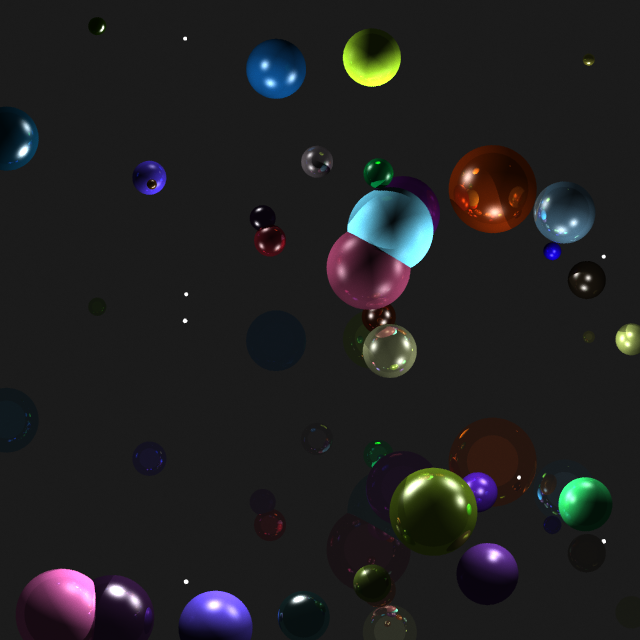
\includegraphics[scale=0.45]{cover.png} 
		\end{center}
	
    
        \HRule\\[0.5cm]
        { \large \today }
    \end{center}
\end{titlepage}

\begin{abstract}

The need for higher quality and faster computer rendering has been demanded by many industries since the first CGI images were rendered.  Many different algorithms have been devised over the last few decades but two algorithms have become dominant.  Z-buffering -- the most widely used algorithm -- can render large complex scenes quickly but lacks the ability to render highly realistic lighting.  Ray tracing can produce life-like images with stunning lighting, but more computationally demanding

My proposal is to design and develop a real-time ray tracer using CPU-based parallel processing.  I plan on investigating several data structures to reduce ray collision testing and minimize algorithm runtime.  The algorithm will be tested with a simple game that will demonstrate the engine's capabilities.  I will also explore utilizing SIMD with Intel's SSE instructions, use the GPU, and distributing the work load over several machines on a network.

\end{abstract}
%\newpage 
%\tableofcontents
\newpage 

\section{ Introduction }
Computer graphics has push the need for faster hardware,  and more efficient algorithms and data structures.  Producing life-like computer-generated images,  computer interfaces, computer-aided design in manufacturing, a multi-billion dollar game industry, and life-like CGI movies\cite{gaming:2007} has made computer graphics an important field of study.

There are two dominant rendering algorithms in computer graphics.  The most widely used algorithm is the z-buffer, which is based upon sorting triangles in a depth buffer.  The other algorithm is ray casting that is based on the physics of light.  Both algorithms are commonly used today, but often for different purposes.  

\section{Z-Buffering}

Computer graphics used in modern games and simulation environments that require real time updates to its environment are based around the z-buffering algorithm.  Z-buffering builds a scene by computing the depth of triangles in a scene from a view-point,  known as the eye.  The algorithm is simple and each pixel can be computed with stream processors that are commonly  used on modern GPUs.  Hardware implementations of z-buffers commonly have two frame buffers for color and a depth buffer.    The color buffer is split into the front buffer and the back buffer.  The back buffer is where the algorithm is rendering to, and the front buffer is drawn to the screen.  Once the back buffer is filled it is swapped with the front buffer,  -- normally done with a simple pointer swap.  The algorithm for z-buffer is as follows \cite{fast:2008}:

\begin{algorithm}
\begin{algorithmic}[1]
\STATE $C[ ] \gets \textit{background color}$ 
\STATE $Z[ ] \gets \infty$
\FOR{ all \textit{N} triangles }
	\FOR{ each pixel p in triangle }
		\STATE $c \gets \textit{new color}$
		\STATE $z \gets \textit{new depth}$
		\IF{ $z < Z_{p} $ }
			\STATE $Z_{p} \gets z$
			\STATE $C_{p} \gets c$
		\ENDIF
	\ENDFOR
\ENDFOR
\end{algorithmic}
\caption{Example of the z-buffer algorithm}
\label{z-buffer}
\end{algorithm}

This algorithm works by tracking the color depth for each given pixel rendered in the back buffer.  This algorithm is fast and easy to implement.  However light, shadow, reflection, or refraction are not calculated.   Z-buffering only renders from a single point, the eye, but to calculate shadow or reflection the algorithm needs to be able to work from any point in space.  Ray casting is often used to produce these effects.  The solution relies on building a better physics-based model for light.

\section{Ray Tracing}

To make a better model we first need to understand how light works.  In the real world a light source emits photons that collide with an object, which changes the energy state of the photon.  This photon is then reflected off the object and then enters our eyes, which our brain then interprets as a color.  One problem with this modelling is that only a small percent of emitted light is actually seen.  A better more efficient solution exists in using ray tracing.  

Ray tracing model realistic light by tracing photons that enter the eye back the light source.  Each photon can be computed independently which making ray tracing inherently parallel.  An initial point is used as the focal point, again known as the \textit{eye}.  A photon is traced backwards from the eye through an image plane in front of the eye.  This image plane acts like film in a pinhole camera.  

\begin{figure}[H]
\begin{center}
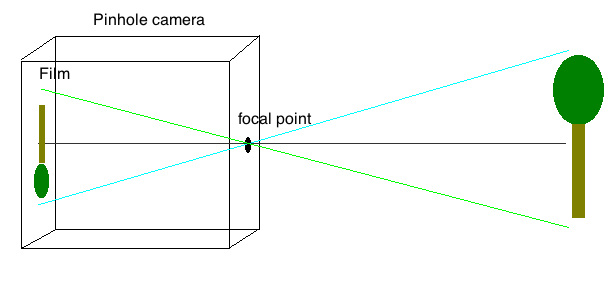
\includegraphics[scale=0.6]{pineholecamera.png} 
\caption{Pinhole camera}
\label{pinhole-camera}
\end{center}
\end{figure}

In a pinhole camera the image is upside down on the film; photons pass through the focal point and cross the central plain.  The camera can be simplified by moving the film in front of the focal point.

 \begin{figure}[H]
 \begin{center}
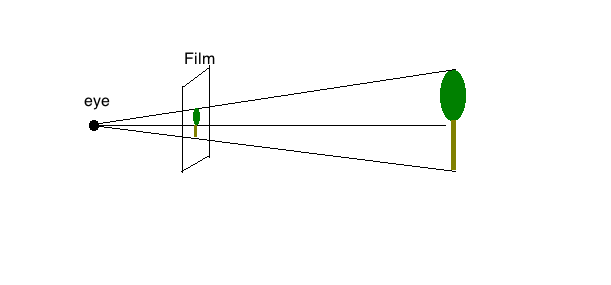
\includegraphics[scale=0.6]{raycamera.png} 
\caption{Ray tracer camera}
\label{ray-camera}
\end{center}
\end{figure}

Algorithm \ref{ray-trace} is a simple implementation producing images similar to the z-buffering algorithm.  The scene consists of a list of geometric objects.  Unlike z-buffering any shaped object can be used.  The image buffer is an array that holds the resulting output colors from the algorithm.  A ray consists of a starting vector and a normalized direction vector.  A ray is created at the eye/starting vector in the direction of each pixel in the image plane.  The pixel is set to the color of the closest object that collides with the ray.  

\begin{algorithm}[H]
\begin{algorithmic}[1]
\STATE $O[ ] \gets \textit{All objects in scene}$ 
\STATE $I[] \gets 0$ \COMMENT{Clear image buffer}
\STATE
\FOR{ each pixel p in I }
	\STATE $I_{p} \gets raytrace( castray( eye, p ))$
\ENDFOR
\STATE 
\STATE \textit{color} \textbf{function} raytrace(  R )
	\STATE $c  \gets \textit{ambient color } $
	\STATE $d \gets \infty $
	\FOR{ each object o in O[] }
		\IF{ collision( R, o )  }
			\IF{ $distance( \textit{eye}, o ) < d$ }
				\STATE $d \gets distance( \textit{eye}, o )$
				\STATE $c \gets color( o )$
			\ENDIF
		\ENDIF
	\ENDFOR
	\STATE \textbf{return} c

\end{algorithmic}
\caption{Simple ray tracing algorithm.}
\label{ray-trace}
\end{algorithm}

Adding light and shadow with this algorithm is done by computing the amount of light at each point of collision.  A ray is cast from each collision point to every light source in the scene.  Any object between the collision point and the light is in shadow.   It does not get light added to its color. If the ray's closest collision is with the light source then the point's color is computed.  A point's color is computed from three components: \textit{ambient}, \textit{diffuse}, and \textit{specular} lighting\cite{kalinini:2008}.

Surfaces can be made reflective or refractive by using recursion.  If a surface is reflective a new ray is computed at the point of collision.   The surface normal at that point  is used as a reflection plane to create the reflected ray.  This new ray is used to compute reflected color.  This produces shiny surfaces and mirrors.  

Refraction is handled in the same way with the exception of the way the refracted ray is computed.  Refracted rays are bent into the object.  The angle depends on the properties of the object's material.  Light passing through transparent materials like glass and water. Algorithm \ref{ray-trace-full} shows an example program using lighting, reflections, and refractions.
  
\begin{algorithm}[H]
\begin{algorithmic}[1]
\STATE $O[\ ] \gets \textit{All objects in scene}$ 
\STATE $L[\ ] \gets \textit{All lights in scene}$
\STATE $I[\ ] \gets 0$ \COMMENT{Clear image buffer}
\STATE
\FOR{ each pixel p in I }
	\STATE $I_{p} \gets raytrace( castray( eye, p ))$
\ENDFOR
\STATE 
\STATE \textit{color} \textbf{function} raytrace(  R, depth )
	\STATE $c  \gets \textit{ambient color } $
	\STATE $d \gets \infty $
	\STATE $s \gets \textit{NULL}$
	\FOR{ each object o in O[] }
		\IF{ collision( R, o )  }
			\IF{ $distance( \textit{eye}, o ) < d$ }
				\STATE $d \gets distance( \textit{eye}, o )$
				\STATE $s \gets o$
			\ENDIF
		\ENDIF
	\ENDFOR
	\IF{ $s\ \textbf{NOT}\ \textit{NULL}$ }
		\STATE \COMMENT{Find direct light on object s}
		\STATE $pi \gets pointOfCollision( R, s )$
		\FOR{ each light l in L }
			\STATE $lr \gets castRay( pi, l )$
			\STATE $ld \gets distance( pi, l )$
			\STATE $shade \gets 1$
			\FOR{ each object o in O }
				\IF{ collision( lr, o ) \textbf{AND} distance( lr, o ) < ld }
					\STATE $shade \gets 0$				
				\ENDIF
				\STATE $c \gets c +( diffuse( s, l ) + specular( s, l )) * shade$ 
			\ENDFOR
		\ENDFOR
		\STATE \COMMENT{Recursively compute reflections}
		\IF{ $reflectivity( s ) > 0\ \textbf{AND}\ depth < depthMax$ }
			\STATE $rr \gets reflection( pi, normal( s, pi ))$
			\STATE $c \gets c + raytrace( rr ) * reflectivity( s )$
		\ENDIF
		\STATE \COMMENT{Recursively compute refraction}
		\IF{ $transparency( s ) > 0\ \textbf{AND}\ depth < depthMax$ }
			\STATE $rr \gets refraction( pi, normal( s, pi ), s )$
			\STATE $c \gets c + raytrace( rr ) * transparency( s )$
		\ENDIF
	\ENDIF
	\STATE \textbf{return} c

\end{algorithmic}
\caption{ Ray tracing algorithm with lighting. }
\label{ray-trace-full}
\end{algorithm}
\newpage

Images produced with this algorithm tend to have overly sharp edges between objects and shadows, and pixelation.  Anti-aliasing is used to reduce jagged edges and pixelated objects. Soft shadows reduces the sharp transition from light to shadow.

Anti-aliasing is done by casting more rays through a pixel and averaging the resulting colors.  The area in space a pixel occupies is subdivided into smaller regions.  Rays are cast from the eye through these regions.  Rays can be cast through the center for a shaper image, or randomly for softer edges.  Anti-aliasing can increase the computation cost dramatically.  Each new ray can create two new rays for reflection and refraction.

\begin{figure}[H]
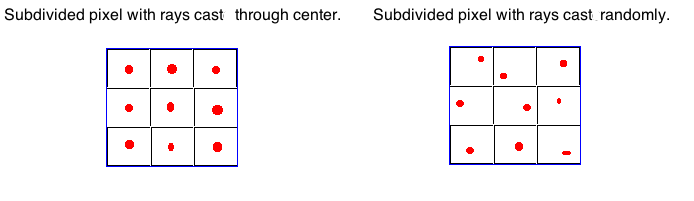
\includegraphics[scale=0.6]{aa.png} 
\caption{Anti-aliasing for a single pixel.}
\label{aa}
\end{figure}

 The simple lighting model casts a ray from the point of collision to the center of a light source, however points on the edge of a shadow may be in partial light.  In the real world a light bulb has volume unlike a single point.  A soft shadow is computed by casting several rays from the collision point to a point in the light's volume, the results are averaged to computer the final color.  These rays are often cast randomly through a uniform subdivision of the light source's volume.  Most ray tracers only use soft shadowing on simple shapes like planes and polygons.  Soft shadows can be expensive to compute because each light ray needs to be tested if it is blocked by an object.

\begin{figure}[H]
\begin{center}
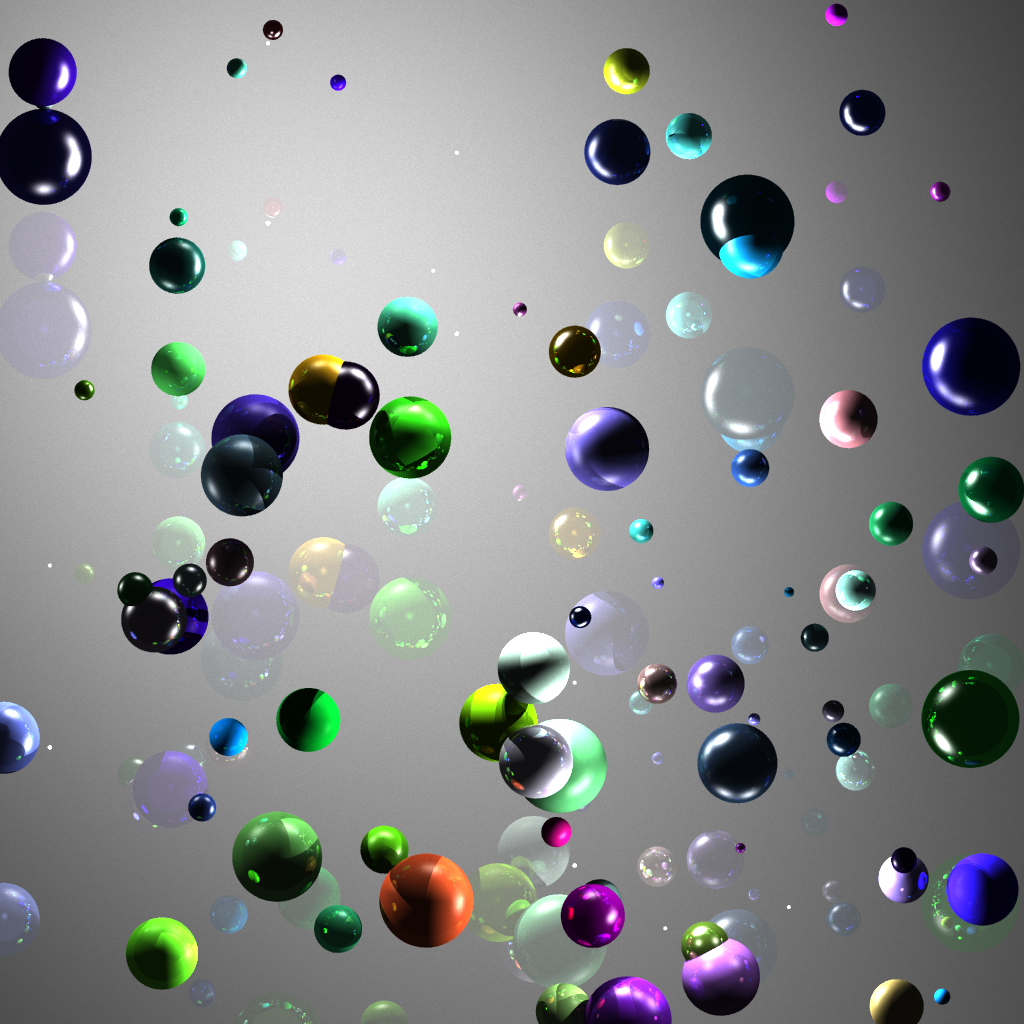
\includegraphics[scale=0.21]{result1.png} 
\caption{Non-optimized ray-traced image with eight light sources, and eighty spheres.  Rendering time was thirty-four minutes .}
\label{result1}
\end{center}
\end{figure}

\section{Run Time Complexity}
The runtime of algorithm \ref{ray-trace} can be computed as $O(n^2)$.    The ray trace function iterates over all objects in the scene to test for a ray-object collision.  The ray trace function is called for every pixel in the output image.   The algorithm can be improved by using a different data structure to store the scene's objects and lights.

The runtime of the full ray tracer algorithm \ref{ray-trace-full} is more complex to compute.  Without recursive calls the ray trace function has a $O(n^2 + n^3 )$.  This changes when we allow for recursion.  Each ray can cast two more rays up to a set maximum depth.  The maximum depth prevents infinite recursion and can control the algorithms performance.  This leaves us with a runtime of $O(2kn^2+2kn^3)$.  Adding soft shadows and anti aliasing can make this even more complex.

Using linear lists of objects and lights creates a serious performance hit.  Using a data structures that reduces the number of objects tested for ray-object collisions will give a dramatic performance boost to the algorithm.


\section{Real-time}
I am proposing to implement a real-time ray tracer.  I will research algorithms and data structures to reduce the ray tracer run time.  I will research techniques of CPU parallelism for algorithms and data structures.  I believe it is possible to reduce the algorithms runtime with either parallel ray casting or parallel collision detection.

Much of the research in real-time ray tracing is concentrated around fast ray-object collision testing.  One of the simplest ways to speed this up is by reducing the number of collision tests\cite{kd:2005}.
Much of this research is about parallel kd-tree ray tracing on the GPU\cite{kd:2007}\cite{fkd:2007}.  I believe much of this research can be applied to fast CPU-based kd-tree ray tracing\cite{kd:2006}.

I plan to design a simple game world to test the ray tracer.  The game world will contain several areas that will test different aspects of the algorithm, as well as areas that will test performance.  The goal of the game world will be to have an $800x600$ screen resolution run at $24$ frames per second.  The test-bed machine will be a $2.2 GHz$ Intel Core i7 MacBook Pro with $8GB$ of RAM.  

\newpage
\listofalgorithms
\listoffigures
%\listoftables
\bibliographystyle{plain}
\bibliography{proposal}

\end{document}

